\documentclass{standalone}
%outline around text
\usepackage[outline]{contour}
\contourlength{1.3pt}

%tikz
\usepackage{tikz}
\usetikzlibrary{knots, cd, calc}

\begin{document}


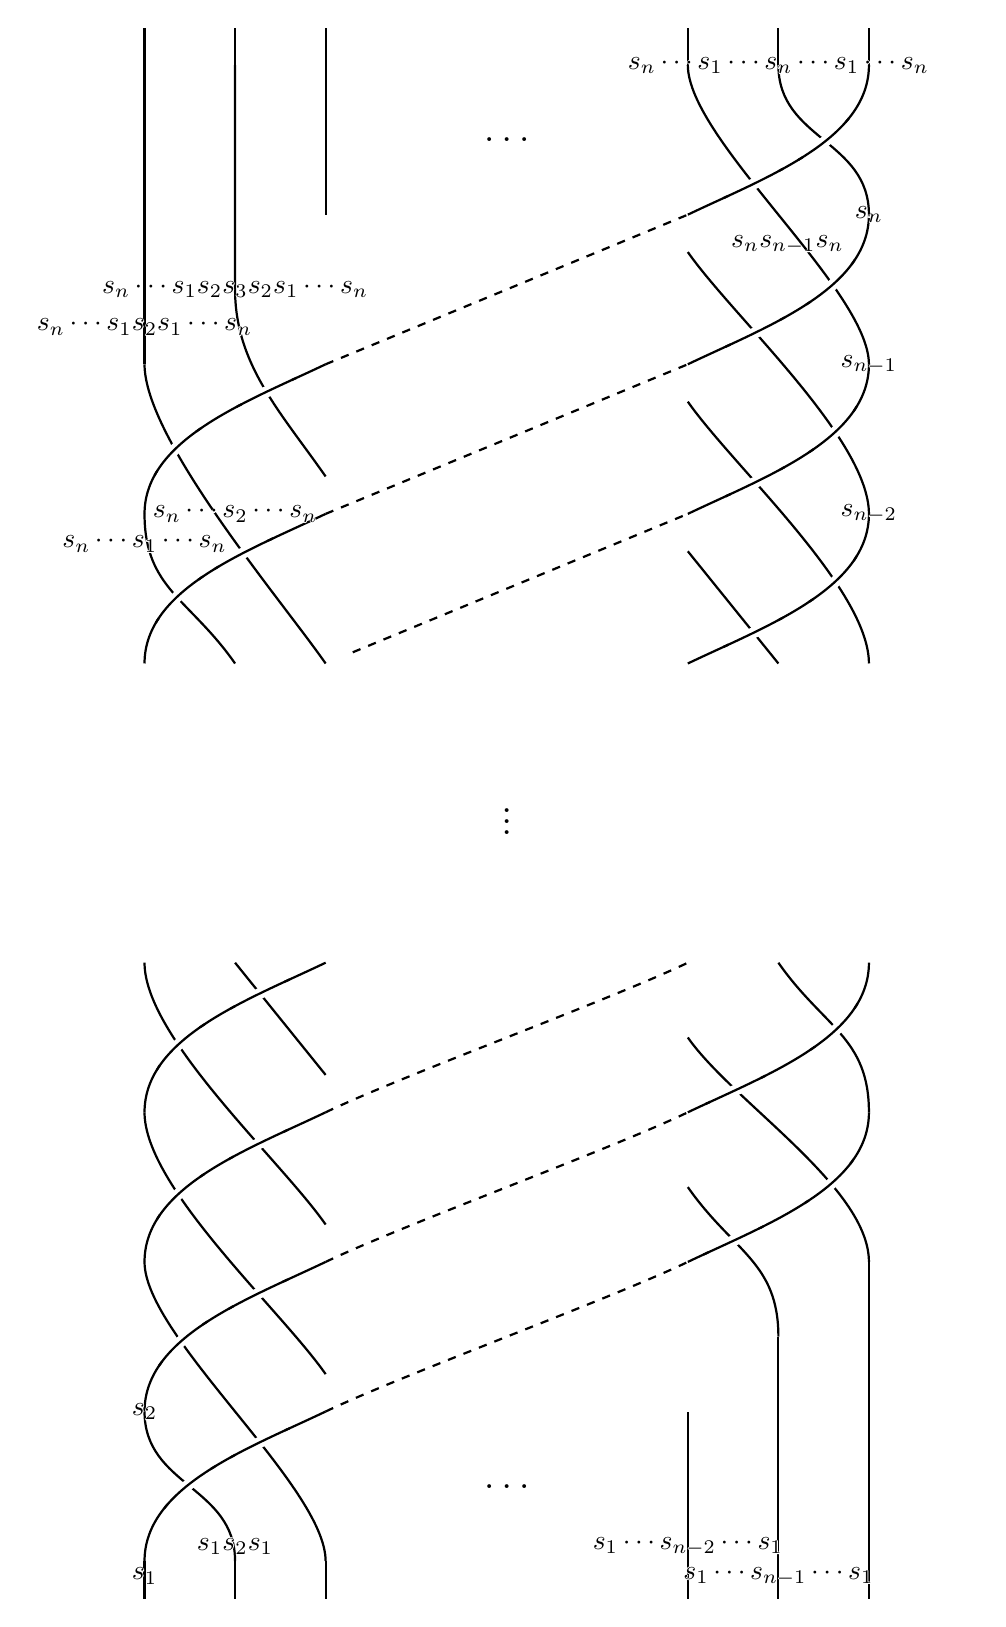
\begin{tikzpicture}[yscale=0.95, xscale=1.15]
\begin{knot}[clip width = 5]
\clip (-1.2, -0.5) rectangle (9.2, 20.5);
\strand[thick] (0, 0) .. controls +(0,1) and +(30:-1) .. (2, 2);

\strand[thick, dashed] 
	(2, 2) .. controls +(30:1) and +(30:-1) .. (6, 4);
	
\strand[thick] 
	(6, 4) .. controls +(30:1) and +(0, -1) .. (8, 6);
	
\strand[thick] 
	(1, 0) .. controls +(0, 1) and +(0, -1) .. (0, 2);

\strand[thick] (0, 2) .. controls +(0,1) and +(30:-1) .. (2, 4);

\strand[thick, dashed] 
	(2, 4) .. controls +(30:1) and +(30:-1) .. (6, 6);
	
\strand[thick] 
	(6, 6) .. controls +(30:1) and +(0, -1) .. (8, 8);
	
\strand[thick] 
	(2, 0) .. controls +(0, 1) and +(0, -1) .. (0, 4);

\strand[thick] (0, 4) .. controls +(0,1) and +(30:-1) .. (2, 6);

\strand[thick, dashed] 
	(2, 6) .. controls +(30:1) and +(30:-1) .. (6, 8);

\strand[thick] 
	(0, 6) .. controls +(0, 1) and +(30:-1) .. (2, 8);

\strand[thick] (6, 0) -- (6, 2);
\strand[thick] (7, 0) -- (7, 3);
	
\strand[thick] 
	(7, 3) .. controls +(0, 1) and +(120:-1) .. (6, 5);
	
\strand[thick] (8, 0) -- (8, 4);
\strand[thick] 
	(8, 4) .. controls +(0, 1) and +(120:-1) .. (6, 7);
	
\strand[thick] 
	(8, 6) .. controls +(0, 1) and +(120:-1) .. (7, 8);

\strand[thick] (2, 6.5) -- (1, 8);

\strand[thick] 
	(2, 2.5) .. controls +(120:1) and +(0, -1) .. (0, 6);
	
\strand[thick] 
	(2, 4.5) .. controls +(120:1) and +(0, -1) .. (0, 8);

\strand[thick] 
	(0, 12) .. controls +(0,1) and +(30:-1) .. (2, 14);
	
\strand[thick, dashed] (2, 14) -- (6, 16);

\strand[thick] 
	(6, 16) .. controls +(30:1) and +(0, -1) .. (8, 18);


\strand[thick] 
	(0, 14) .. controls +(0,1) and +(30:-1) .. (2, 16);
	
\strand[thick, dashed] (2, 16) -- (6, 18);

\strand[thick] 
	(6, 18) .. controls +(30:1) and +(0, -1) .. (8, 20);
	
\strand[thick] 
	(1, 12) .. controls +(120:1) and +(0, -1) .. (0, 14);
	
\strand[thick] 
	(2, 12) .. controls +(120:1) and +(0, -1) .. (0, 16);
	
\strand[thick] (0, 16) -- (0, 20);



\strand[thick] 
	(2, 14.5) .. controls +(120:1) and +(0,-1) .. 
	(1, 17) -- (1, 20);
	
\strand[thick] (2, 18) -- (2, 20);

\strand[thick, dashed] (2.3, 12.15) -- (6, 14);

\strand[thick] 
	(6, 14) .. controls +(30:1) and +(0, -1) .. (8, 16);
	
\strand[thick] 
	(6, 12) .. controls +(30:1) and +(0, -1) .. (8, 14);

\strand[thick] 
	(8, 18) .. controls +(0, 1) and +(0, -1) .. (7, 20);
	
\strand[thick] 
	(8, 16) .. controls +(0, 1) and +(0, -1) .. (6, 20);
	
\strand[thick] 
	(8, 14) .. controls +(0, 1) and +(120:-1) .. (6, 17.5);
	
\strand[thick] 
	(8, 12) .. controls +(0, 1) and +(120:-1) .. (6, 15.5);
	
\strand[thick] (7, 12) -- (6, 13.5);

%tails
\strand[thick] (0, 20) -- +(0, 0.5);
\strand[thick] (1, 20) -- +(0, 0.5);
\strand[thick] (2, 20) -- +(0, 0.5);
\strand[thick] (6, 20) -- +(0, 0.5);
\strand[thick] (7, 20) -- +(0, 0.5);
\strand[thick] (8, 20) -- +(0, 0.5);

\strand[thick] (0, 0) -- +(0, -0.5);
\strand[thick] (1, 0) -- +(0, -0.5);
\strand[thick] (2, 0) -- +(0, -0.5);
\strand[thick] (6, 0) -- +(0, -0.5);
\strand[thick] (7, 0) -- +(0, -0.5);
\strand[thick] (8, 0) -- +(0, -0.5);
\end{knot}

\node at (4, 1) {\Large{$\dots$}};
\node at (4, 19) {\Large{$\dots$}};
\node at (4, 10) {\Large{$\vdots$}};

\node at (0, -0.2) {\contour{white}{$s_1$}};
\node at (0, 2) {\contour{white}{$s_2$}};
%\node at (0, 4) {\contour{white}{$s_3$}};

\node at (1, 0.2) {\contour{white}{$s_1s_2s_1$}};
%\node at (1, 2) {\contour{white}{$s_2s_3s_2$}};
%\node at(2, 0.2) {\contour{white}{$s_1s_2s_3s_2s_1$}};
\node at (6, 0.2) {\contour{white}{$s_1 \cdots s_{n-2} \cdots s_1$}};
\node at (7, -0.2) {\contour{white}{$s_1 \cdots s_{n-1} \cdots s_1$}};
%\node at (0, 10) {\contour{white}{$s_n$}};
\node at (8, 16) {\contour{white}{$s_{n-1}$}};
\node at (8, 14) {\contour{white}{$s_{n-2}$}};
%\node at (8, 10) {\contour{white}{$s_{n-3}$}};
%\node at (7.5, 13.6) {\contour{white}{$s_{n-1}s_{n-2}s_{n-1}$}};
%\node at (6.4, 13.2) {\contour{white}{$s_{n-1}s_{n-2}s_{n-3}s_{n-2}s_{n-1}$}};

\node at (8, 18) {\contour{white}{$s_n$}};
\node at (7.1, 17.6) {\contour{white}{$s_ns_{n-1}s_n$}};
\node at (0, 13.6) {\contour{white}{$s_n\cdots s_1 \cdots s_n$}};
\node at (1, 14) {\contour{white}{$s_n \cdots s_2 \cdots s_n$}};

\node at (0, 16.5) {\contour{white}{$s_n \cdots s_1 s_ 2 s_ 1 \cdots s_n$}};
\node at (1, 17) {\contour{white}{$s_n \cdots s_1 s_ 2 s_3 s_2 s_1 \cdots s_n$}};
\node at (7, 20) {\contour{white}{$s_n \cdots s_1 \cdots s_n \cdots s_1 \cdots s_n$}};

\end{tikzpicture}

\end{document}
